\documentclass[11pt]{article}
\title{\textbf{Perceptions \& Use of BitTorrent P2P File Sharing by Dartmouth College Students\footnote{This paper constitutes the final project for the Fall 2013 iteration of CS 55: Security and Privacy, taught by Charles C. Palmer, Adjunct Professor of Computer Science, Dartmouth College; CTO Security and Privacy, IBM Research.}}}
\author{
	Alex Gerstein \\ Dartmouth College\\ Computer Science \\ \texttt{alex.gerstein@dartmouth.edu} 
	\\ \\
	Scott Gladstone \\ Dartmouth College\\ Computer Science, Economics\\ \texttt{scott.gladstone@dartmouth.edu}
	}
\date{\today}

\usepackage[margin=1.0in]{geometry}
\setlength{\parskip}{10pt plus 1pt minus 1pt}
\usepackage{fancyhdr}
\usepackage{enumerate}
\usepackage{multicol}
\usepackage{fixltx2e}
\usepackage{graphicx}
\usepackage[font=small,labelfont=bf]{caption}
\usepackage[superscript,biblabel]{cite}
\usepackage{url}


\begin{document}

\maketitle
\begin{abstract}
In our final project, we investigated student perceptions and use of the BitTorrent peer-to-peer (P2P) file-sharing protocol at Dartmouth College. After a general overview of the protocol, potential legal implications, and security flaws present, we surveyed students and spoke to Adam Goldstein at Dartmouth College Computing Services in order to better understand the disparity between the perception and actual use of torrenting by students. Using the results from the survey and network bandwidth data obtained from Computing Services, we observed several notable sources of disconnect between student perceptions and incidences of torrenting. These disparities include a perception by students that the average Dartmouth student torrents more then than the student participants actually reported, the observation that the number of DMCA complaints far understates the number of students who illegally torrent, and the fact that BitTorrent is still the most utilized file-sharing service at Dartmouth College despite the rise of alternative forms of media management such as video- and audio-streaming services like Netflix and Spotify. This paper outlines the goals, methods, and results of our study and discusses potential policy recommendations for the College in order to curb illegal torrenting and reduce the vulnerability of the Dartmouth College network to torrent-related exploits.
\end{abstract}

%%%%%%%%%%%%%%%%%%%%%%%%%%%%%%%%%%%
%%%% ********			INTRODUCTION  		******** %%%%%
%%%%%%%%%%%%%%%%%%%%%%%%%%%%%%%%%%%

\pagebreak
\section{Introduction}

BitTorrent is a protocol supporting peer-to-peer (P2P) file sharing that facilitates the distribution of large data files over the Internet \cite{BitTorrent}. BitTorrent is one of the most common protocols for transferring large files and is often used to distribute popular files and files available for free, such as literary texts, audio files, movies, and applications. ``Torrenting'' is the process by which a user engages with a BitTorrent client in order to send and receive those desired files. To understand the uniqueness -- and security implications -- of the BitTorrent protocol, one must first develop a working understanding of P2P file sharing. From there, the legality of P2P file sharing and torrenting can be made clear. With this foundation, the authors conducted a study in which student perceptions of torrenting at Dartmouth College were compared  with Dartmouth College Computing Service's data on student torrenting. Conclusions and policy recommendations are then made with the goal of aligning student perceptions and administrative desires with regard to torrenting. To the best of the authors' knowledge, this is the first study conducted that compared student perceptions and actual incidences of torrenting at Dartmouth College.

\subsection{Peer-to-Peer (P2P) File Sharing}
P2P is a ``type of Internet network that allows users with the same program to connect with each other and access files on one another's hard drives without the intervention of a server computer.'' \cite{NYTimes} This decentralized network architecture consists of individual nodes called \emph{peers} that act as both suppliers and consumers of resources. In P2P networks, tasks are shared among multiple, interconnected peers who each make a portion of their resources -- processing power, disk storage, or network bandwidth -- available to all network participants, without the centralized coordination of a server-client model \cite{scholl}. A comparison of a decentralized-P2P network and a centralized server-based network are presented in Figure 1 and Figure 2 below.

\begin{figure}[h!]
\centering
\begin{minipage}[b]{0.45\linewidth}
	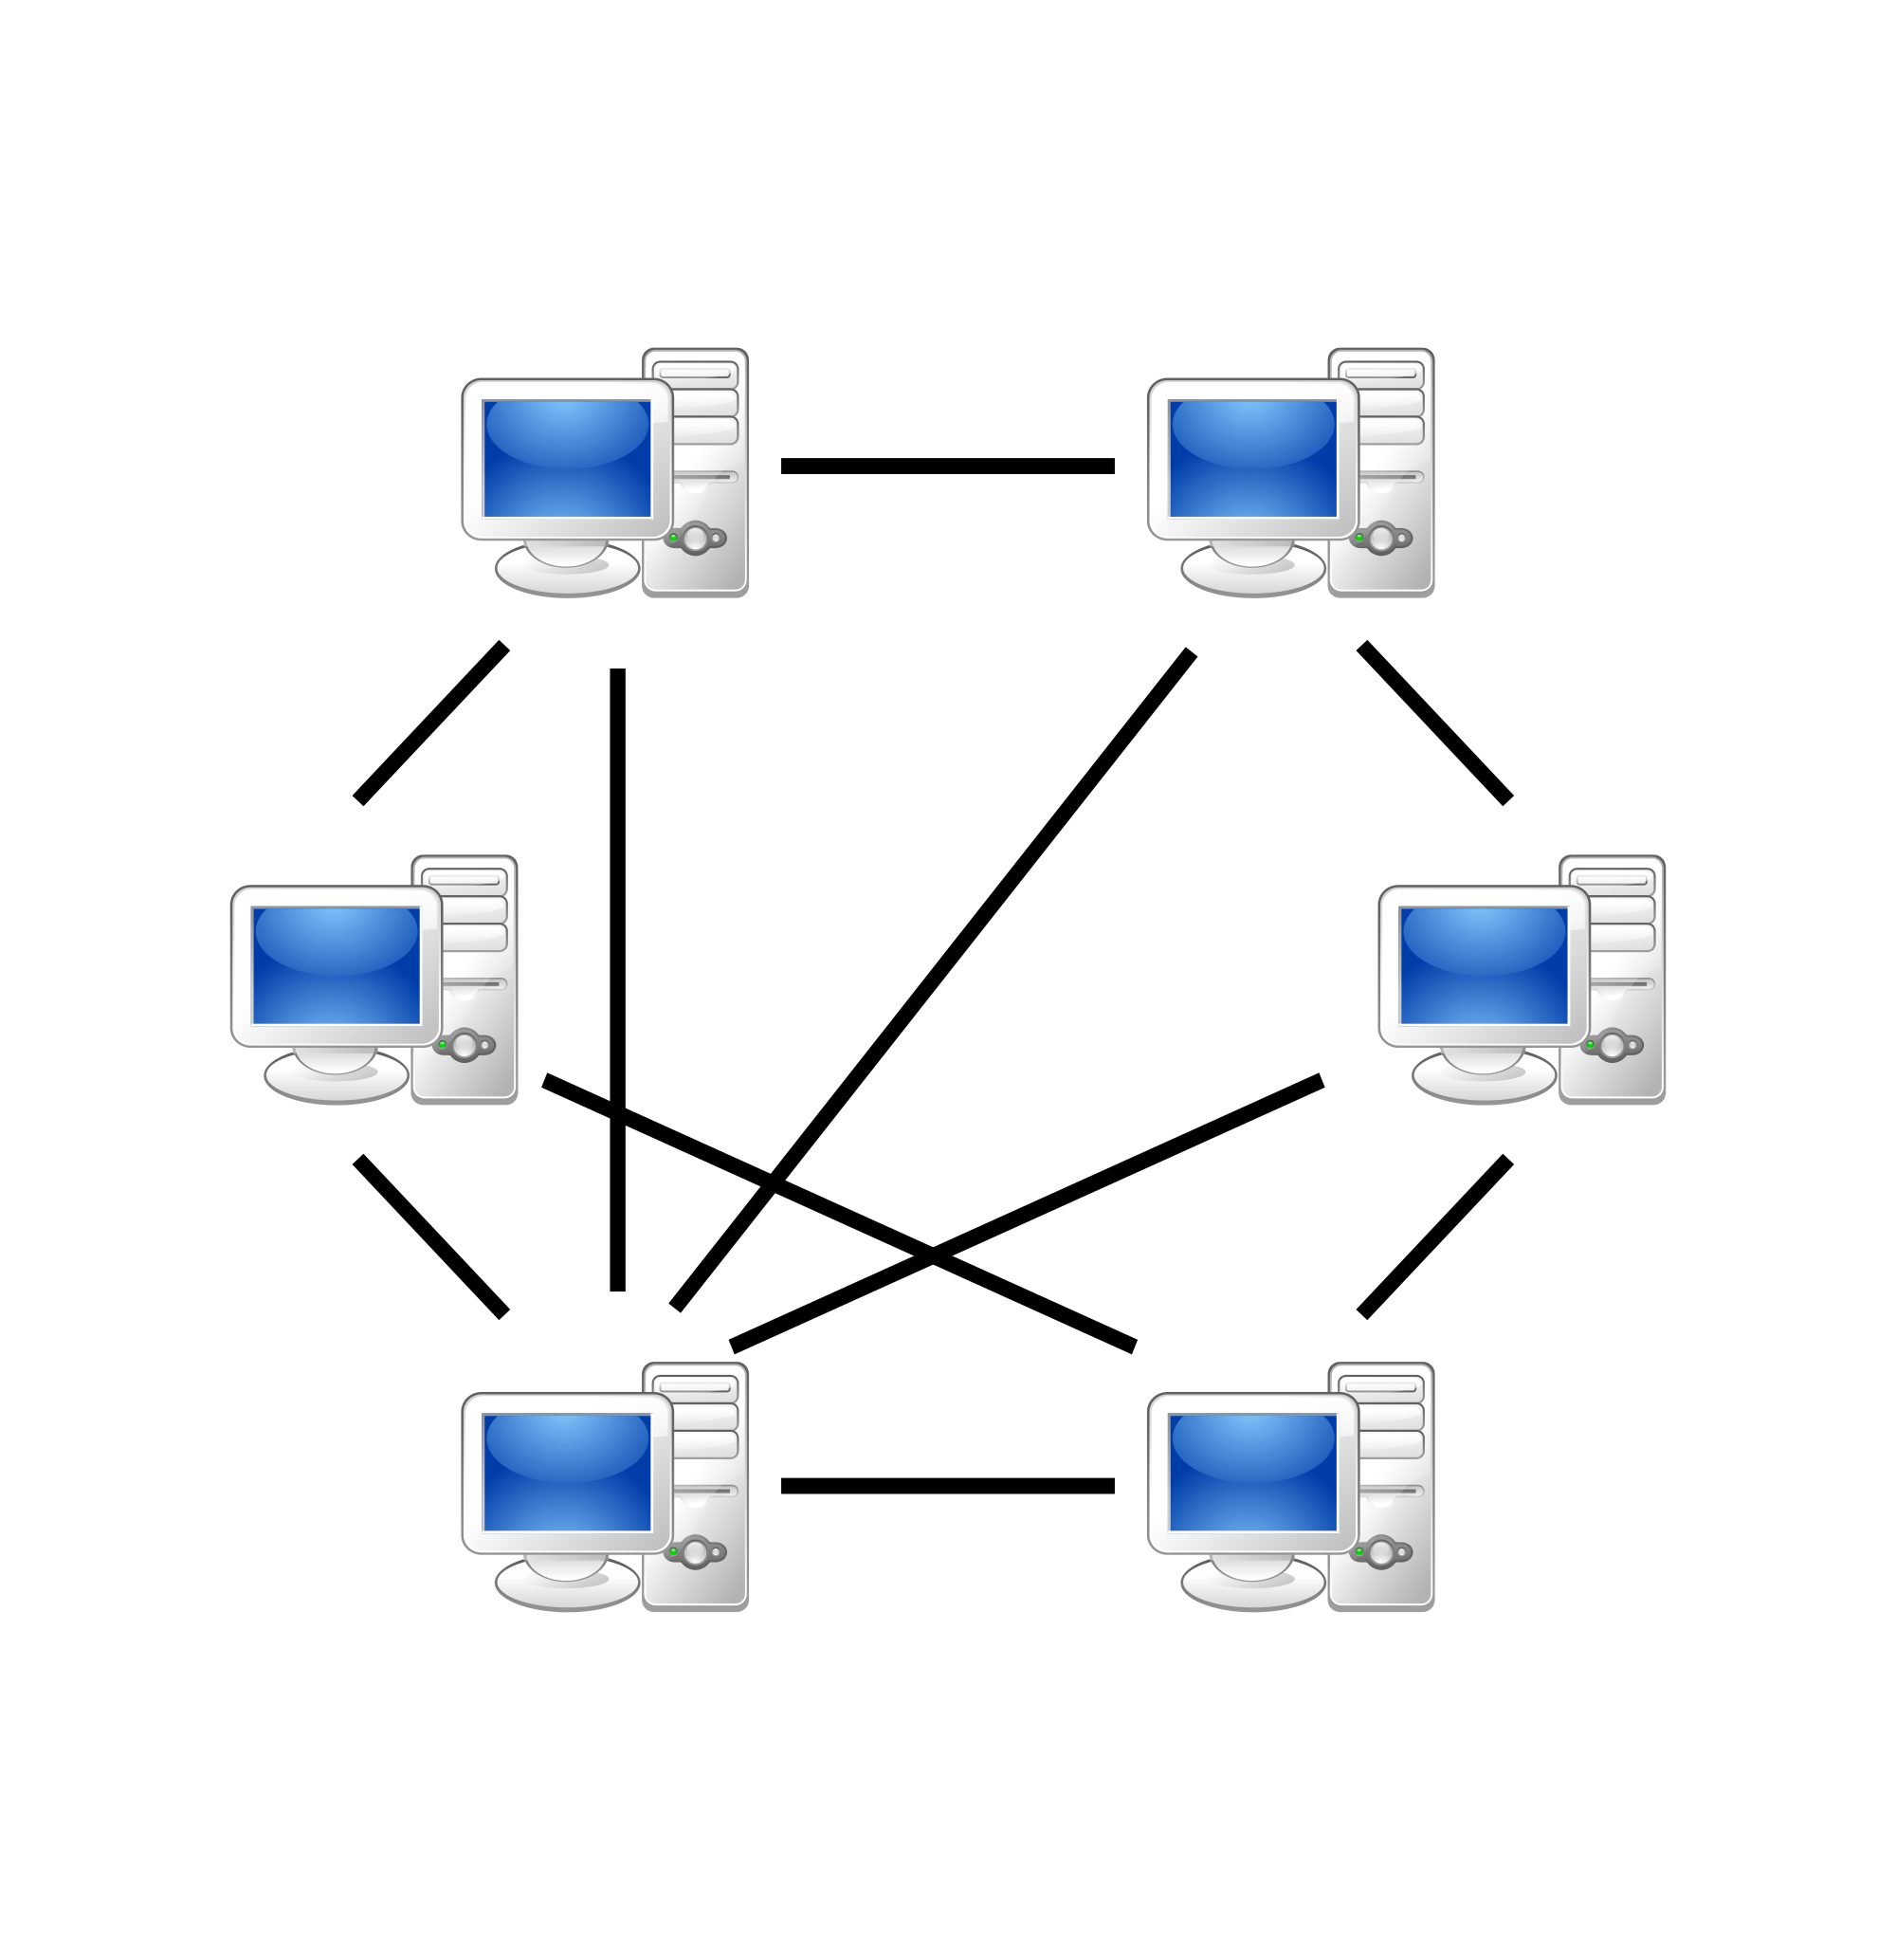
\includegraphics[width=56mm]{P2P-network}
	\caption{A peer-to-peer (P2P) network with interconnected nodes (``peers'') sharing resources. Source: Wikipedia.}
	\label{p2p_network}
\end{minipage}
\quad
\centering
\begin{minipage}[b]{0.45\linewidth}
	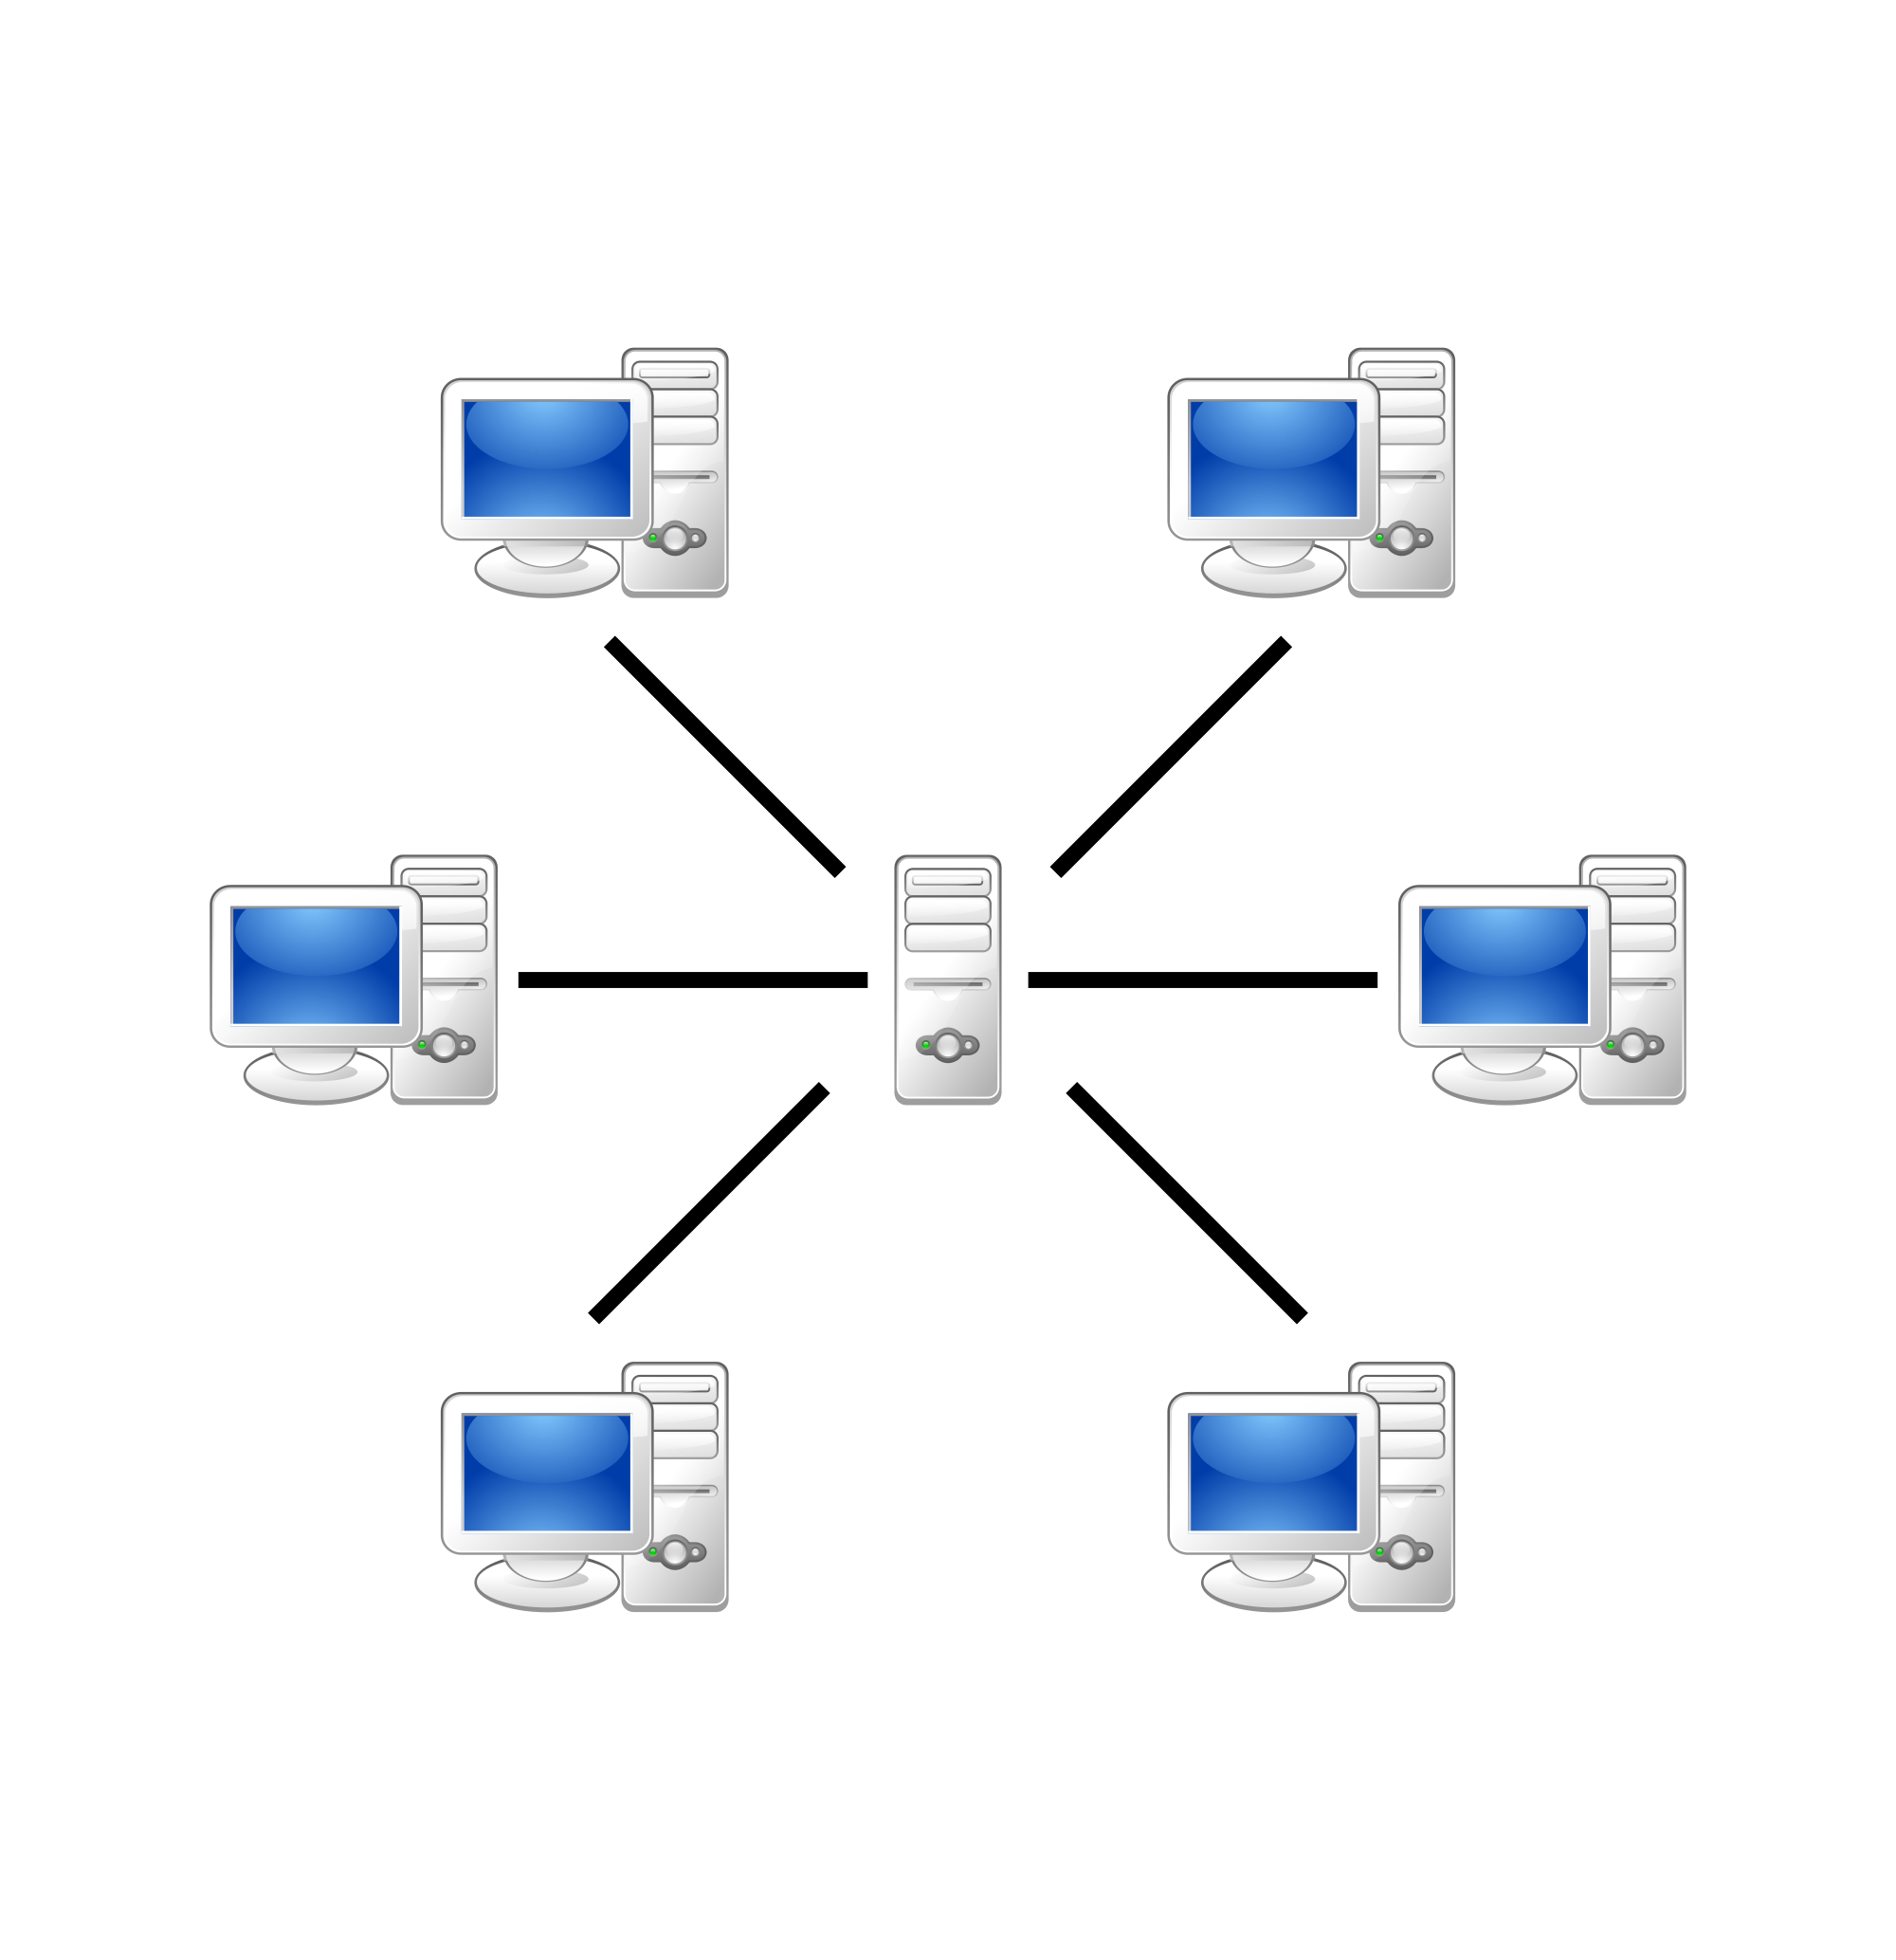
\includegraphics[width=56mm]{Server-based-network}
	\caption{A client-server model network, where individual clients request services from centralized servers. Source: Wikipedia.}
	\label{p2p_network}
\end{minipage}
\end{figure}

P2P networks are often found in residential home networks, allowing users to configure their computers to share files, printers, and other resources among all devices; with a number of computers running similar network protocols, P2P is a convenient way to access shared resources. However, the term ``P2P'' used today generally does not refer to the network architecture from which its name is derived, but to P2P file sharing systems. Using P2P software applications such as Gnutella or eDonkey, users are able to search for, transfer, and download data files over the Internet with any user on the same P2P file sharing network. The implications of such systems are huge: if \emph{any} user on the system has a file that another user demands, the second user can -- via the network -- obtain the file. The second user will then also become a source of the file in the P2P network, making it faster and easier for more users to download the file. 

The first P2P file sharing networks, such as the original iteration of the MP3-sharing network Napster, relied on a central index server to assist with the transfer of files. When someone searched for a file, the central index server -- which contained an index of all of the users and their shared content -- searched for all available copies of the file and presented them to the user; the file would then be transferred directly between the two private computers \cite{P2PFileSharewiki}. Because the file sharing occurred over a central network, Napster was held liable for copyright infringement over the sharing of MP3 files and was shut down in 2001. New protocols such as BitTorrent represent a technological evolution of P2P file-sharing networks.

\subsection{BitTorrent Protocol}

BitTorrent is a P2P file-sharing protocol that makes use of a unique design to reduce the bandwidth and download time for more frequently requested data. The protocol allows users to download a file quickly by integrating all users requesting that file into a ``swarm'' of hosts to download and upload from each other simultaneously. Thus, instead of attempting to transfer a large file from one user to another -- a slow, bandwidth-intensive process -- BitTorrent allows a user to download small segments of the file from a variety of users, significantly reducing computational energy and download time\cite{BitTorrent}. Because of this design, BitTorrent is often used for distribution of very large files, very popular files, and files available for free, as it is more efficient to distribute these files using BitTorrent than a regular download.

When a user ``torrents,'' or attempts to download a file over a P2P network using a BitTorrent client, they begin by loading a .torrent file into the BitTorrent client. A .torrent file is a computer file that contains metadata about the files to be distributed, including file names, sizes, checksums of all individual pieces, and a list of the network locations of ``trackers.'' Trackers are servers that facilitate communication between peers seeking to download the same data on a P2P network \cite{Incentives}. The tracker shares the peers' IP addresses with other BitTorrent clients in the ``swarm,'' the group of all peers sharing a torrent. Each piece of a file specified in a torrent is protected by a cryptographic hash contained in the .torrent file \cite{BitTorrent}. This ensures that any modification of the piece can be easily detected, preventing a user from downloading both accidental and malicious modifications of any pieces of a file.

The process of sharing data via BitTorrent starts with a \emph{seed}, or the initial machine possessing 100\% of the data. Then \emph{leechers}, also known as \emph{downloaders}, load a .torrent file and request a download. Once connected, a BitTorrent client downloads small pieces of the files specified in the torrent from different computers in the swarm. When the BitTorrent client has some data, it can then begin to upload that data to other BitTorrent clients. By using both downloading and uploading bandwidth simultaneously and dividing the files into pieces, the time required to download the file is significantly reduced \cite{BitTorrent}. Thus, it is worth noting that, ``Everyone downloading a torrent is also uploading the same torrent. If 10,000 people are downloading the same file, it doesn't put a lot of stress on [any] central server. Instead, each downloader contributes upload bandwidth to other downloaders, ensuring the torrent stays fast," \cite{HTG}. As the number of downloaders increases, the reliance of new leechers on old sources decreases. Thus, each successful downloader becomes a source of the file for future downloaders \cite{Incentives}. From this point, the process repeats, allowing peers on the network to share any and all files to which any other peer has access.

%%%%%%%%%%%%%%%%%%%%%%%%%%%%%%%%%%%
%%%% ********			LEGAL ISSUES  		******** %%%%%
%%%%%%%%%%%%%%%%%%%%%%%%%%%%%%%%%%%

\section{Legal Issues \& Security Implications}

While the BitTorrent protocol itself is legal, those who use the service often do so to obtain files illegally. Illegally obtaining files, also known as digital piracy, involves sharing copyrighted media such as games, music, movies, TV shows, and software that the user does not have permission to share. Whether the user is downloading or uploading content, involvement in this type of non-permitted operation is considered a violation of copyright law \cite{illegal-downloading}. Often times, digital piracy constitutes a violation of the Digital Millennium Copyright Act (DMCA). The DMCA is a United States copyright law that criminalizes the production and dissemination of technology, devices, or services intended to circumvent digital rights management (DRM) measures that control access to copyrighted works \cite{DMCA}. Penalties for violation include both civil and criminal remedies, which can consist of both significant fines and/or imprisonment. In a 2010 sampling of the one thousand most actively seeded torrent files, 89 percent of the files were confirmed to be illegally shared and the majority of the remaining 11 percent were determined to be ``likely infringing.'' \cite{illegalFilesTorrent} Only three files, or 0.3\%, were confirmed to be legal. The analysis of student's perception of torrenting in this study will focus on the sharing of the illegal torrents, which comprise the overwhelming majority of the data shared through BitTorrent clients.

\subsection{Security Implications for Individuals and Network Hosts}

Whenever a user downloads a file, the downloading device is exposed to major security vulnerabilities. With the BitTorrent protocol, where one torrent often contains links to multiple files, users must be cautious about what they are storing onto their hard drives. The distributed nature of torrents allows for them to be intentionally corrupted, either by anti-piracy groups or malicious attackers.

The entertainment industry and various anti-piracy groups have made numerous attempts to thwart those who torrent illegally. These methods, referred to collectively as torrent poisoning, are effective in both slowing download speeds and gathering IP addresses of the downloaders \cite{torrent-poisoning}. Organizations pose as seeders of a torrent to connect to leechers, or downloaders. Once this connection is made, the anti-piracy organization can save the user's IP address and use various exploits to deter the user from downloading or sharing the file. Counterpiracy companies, such as the now defunct MediaDefender, slow the download of files through numerous methods. These methods are mostly based on seeding or linking to fake files. For example, in a decoy insertion, corrupted versions of a file are distributed on a network to appear indistinguishable from the original files. Attempting to download these files often leads to excessive download times and potential insertion of malware into a user's computer. While a decoy insertion targets the torrent files, a spoofing attack targets the locations of torrents to redirect potential leechers to non-existent locations. Spoofing attacks aim at consuming all of a BitTorrent client's bandwidth resources by having the client to try to grab a file that doesn't exist, thus preventing the user from downloading or uploading any other files. \cite{torrent-poisoning}

Both these attacks are founded on the principle that some downloaders will stop torrenting out of frustration with slow download speeds and corrupted files. However, sometimes copyright enforcers take extreme measures to proactively prevent BitTorrenting. In 2007, Comcast was accused of hindering the uploading of complete files to BitTorrent. In an effort to increase network access speeds, Comcast blocked torrenting applications by using their routers to monitor and prevent certain forms of network traffic. The following year, they were ordered to terminate their ``unreasonable'' network management. In another instance, MediaDefender overstepped their legal rights similarly in 2008 when they caused a Denial of Service attack on Revision3, a legal Internet television network distributor.

However, it is not only the anti-piracy organizations that corrupt torrents. According to multiple studies, BitTorrent is among the most frequently used mechanisms for attackers to distribute malware. One report claims that up to 14.5\% of BitTorrent downloads contain malware and 47\% of all zero-day malware found was distributed through BitTorrent \cite{malware}. With these exploits, attackers are able to execute shell code, install keyloggers, and create zombies on unsuspecting users' computers. 
	
\subsection{Dartmouth College Policy and Practice}

In the "real-world," the legality of torrenting and possible actions an external party can take against torrenters is a little fuzzy. However, when a college student signs an acceptable-use policy to gain access to the campus network, their rights become slightly clearer. In Dartmouth College's "Acceptable Use Policy," users agree to not "post, use, or transmit content that [they] do not have the right to post or use; for example, [content] under intellectual property, confidentiality, privacy or other applicable laws." \cite{AcceptableUsePolicy} Furthermore, Dartmouth's "Copyright Policy \& Guidelines" includes the "copying and sharing images, music, movies, television shows or other copyrighted material through the use of P2P technology" as a probable violation of copyright law. \cite{DartmouthCopyright}

Although the College does not police students' torrenting activities, it often receives formal legal notices from organizations like the Recording Industry Association of America (RIAA) or BayTSP (representer of movie and television studios) for infringers to discontinue their illegal downloading activity. The College is required, by law, to forward these notices to the students responsible. If a user continues his/her behavior after he/she is issued this warning, College Policy states that Dartmouth is permitted to revoke the user's access to its information technology resources. Additionally, any civil or criminal liability pushed by the anti-copyright organizations becomes the liability of the infringing student. In cases filed by the RIAA against students at Princeton, RPI, and Michigan Tech, the recording industry sued for damages of \$150,000 for each recording infringed. In this regard, Dartmouth notes in its copyright policy, ``Dartmouth is not the police; however, Dartmouth will cooperate with law enforcement agencies when required.'' \cite{DartmouthCopyright}

%%%%%%%%%%%%%%%%%%%%%%%%%%%%%%%%%%%
%%%% ********	     METHODS, DATA & ANALYSIS  ******** %%%%%
%%%%%%%%%%%%%%%%%%%%%%%%%%%%%%%%%%%

\section{Methods, Data \& Analysis}
The goals of this research were three-fold: first, to determine the student perception of the occurrence of torrenting at Dartmouth; second, to investigate the actual occurrence of torrenting at Dartmouth based on data provided by Dartmouth College Computing Services; and third, to examine the relationship between student perceptions and actual incidences of torrenting at Dartmouth. The methods employed to carry out these goals and the data collected are described in the sections 3.1 to 3.3.

\subsection{Student Perception Survey}

\subsubsection{Participants}
The participants in the survey were 130 students at Dartmouth College. The population consisted of second-year, third-year, fourth-year, and graduate students at the College. Participation was anonymous and voluntary. All prospective participants were sent a link to a Google Form that contained all of the survey questions. All participants had completely voluntary choice in clicking on the link, examining the questions, and completing and submitting the survey. The population examined in this study may be biased since some individuals who completed the survey may have personally known the researchers or were members of CS 55: Security \& Privacy, the class for which this research was completed.

\subsubsection{Survey Design}
The survey consisted of seven questions, six of which were mandatory. The mandatory questions asked the participant for his/her personal experience with torrenting, whether he/she believed other students at Dartmouth torrented, the number of files that he/she believed the average student torrented, whether he/she believed Dartmouth recorded information about student torrenting, and whether his/her knowledge of Dartmouth Copyright Violation Policy impacted the amount that he/she torrented. The optional seventh question asked whether the participant had any thoughts as to how Dartmouth College could reduce the incidence of torrenting on campus. All surveys were timestamped when submitted and resubmissions/changing of answers were not permitted. See Appendix A for a copy of the survey administered. 

\subsubsection{Perception Data}
Of the 130 students, 78 (60.0\%) stated that they had previously downloaded a file via torrenting. 52 out of 78 individuals (74.3\%) who had torrented in general had also torrented while at Dartmouth. Of the 52 students who designated that they torrented at Dartmouth, 34 (65.4\%) claimed to download one to five files per month on average; 5 (9.6\%) claimed to download zero files per month on average; 5 (9.6\%) claimed to download six to ten files per month on average; and 9 (17.3\%) claimed to download 11 or more files per month on average. 

Considering all 130 students (both torrenters and non-torrenters), 82 (63.1\%) claimed to download zero files per month on average via torrenting. This was statistically significantly different (\emph{p}$<$.00001) from the small percentage of students (16 students, 12.3\%) who reported that they believed that the average Dartmouth student downloads zero files per month via torrenting. The median self-reported number of files downloaded via torrenting on average was zero, while the median perceived number of files torrented by the average student was in the category ``one to five.'' Based on the distributions presented in Figures 3 and 4 below, there is a clear right shift in Figure 4 as compared with Figure 3, indicating that there is likely a significantly higher perception of student torrenting at Dartmouth than what actually occurs.

\begin{figure}[h!]
\centering
\begin{minipage}[b]{0.45\linewidth}
	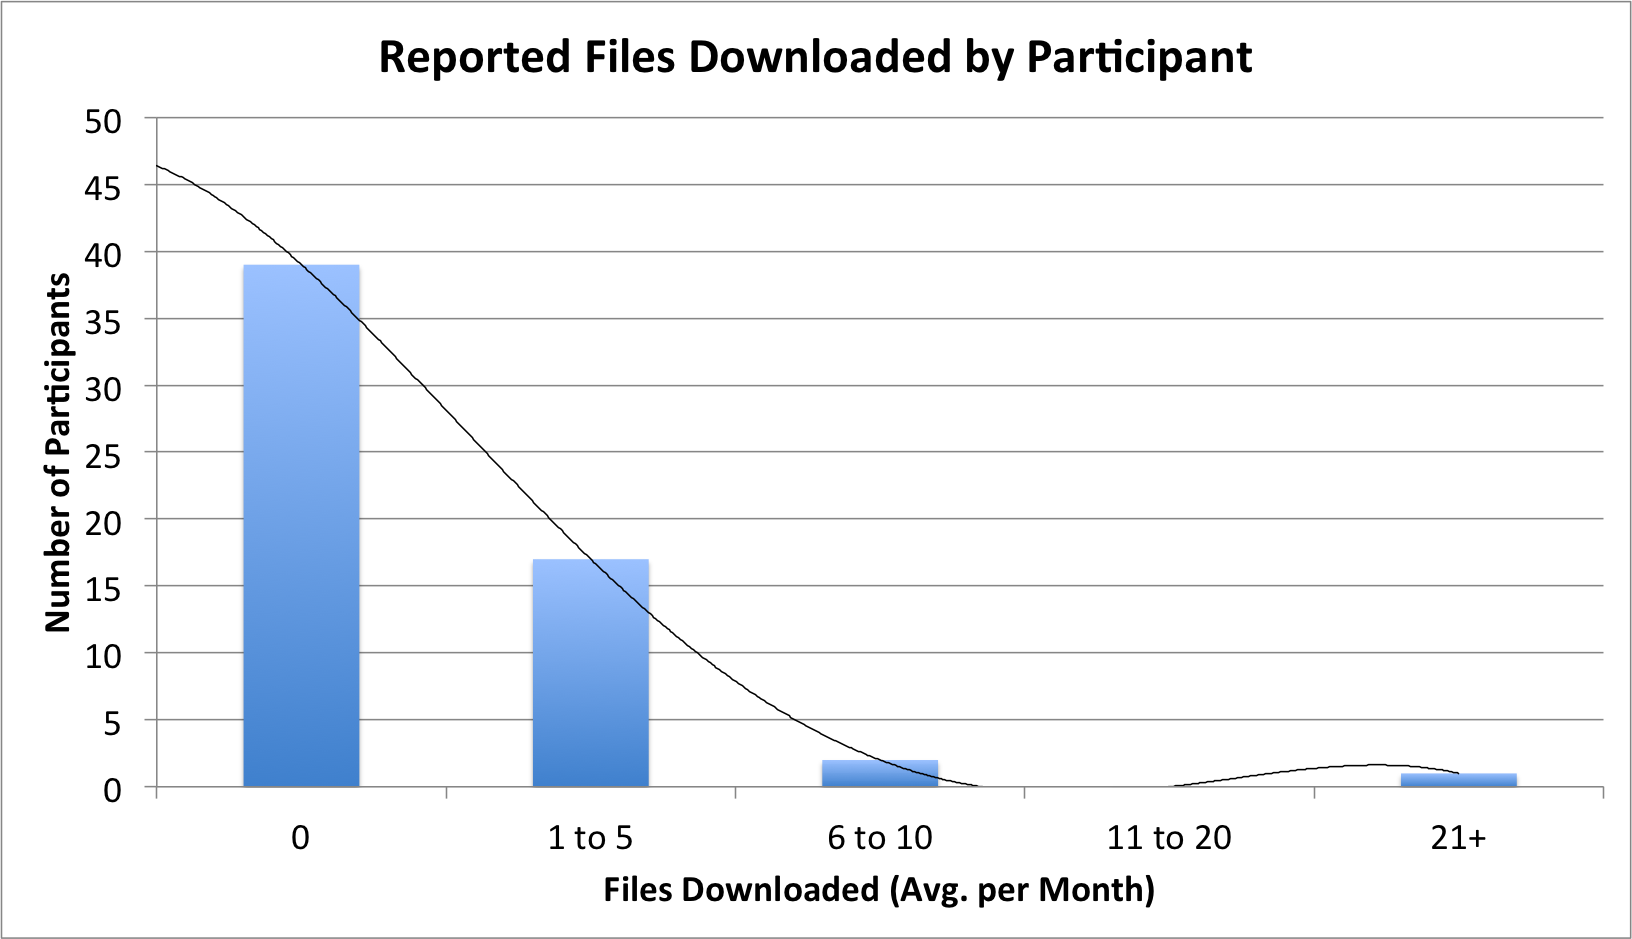
\includegraphics[width=77mm]{Figure3}
	\caption{Bar distribution of reported number of files downloaded via torrenting by the participant.}
	\label{p2p_network}
\end{minipage}
\quad
\centering
\begin{minipage}[b]{0.45\linewidth}
	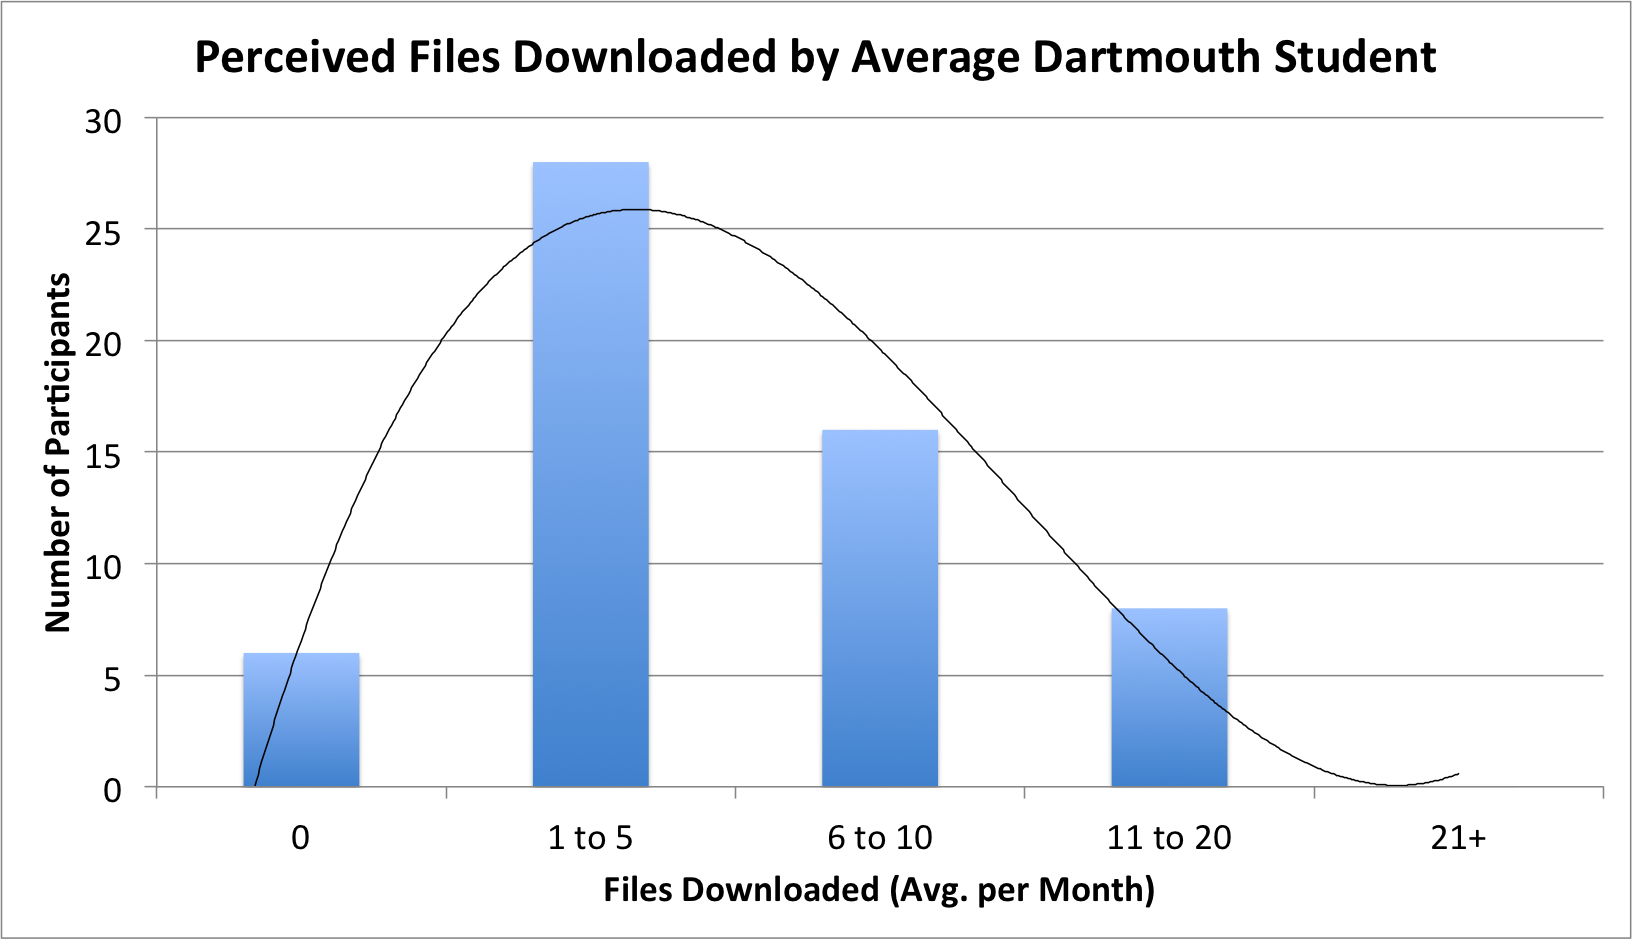
\includegraphics[width=77mm]{Figure4}
	\caption{Bar distribution of perceived number of files downloaded via torrenting by the ``average Dartmouth student.''}
	\label{p2p_network}
\end{minipage}
\end{figure}

The results were less conclusive with regard to whether participants believed that Dartmouth recorded student torrenting information and whether knowledge of Dartmouth's Copyright Violation Policy affects how often the participant torrents. Of the 130 students asked if Dartmouth records when someone torrents a file, 47 (36.2\%) said Yes; 28 (21.5\%) said No; and 55 (42.3\%) said they were Unsure. Attempting to break down the results further by the results of other questions in the survey, the results were still inconclusive. More data would need to be collected to determine this result. Regarding whether knowledge of Dartmouth's Copyright Violation Policy affected personal torrenting practices, there was no significant difference (\emph{p}$>$.05) between the number of participants who said Yes (N=63, 48.5\%) and who said No (N=67, 51.5\%). 

\subsection{Dartmouth Network Patterns}

The researchers in this study met with Adam Goldstein, IT Security Engineer at Dartmouth College Computing Services, to discuss Dartmouth network trends and use of BitTorrent and other file sharing protocols on the Dartmouth network \cite{Goldstein}. Goldstein described the PaloAlto firewall and traffic recording system utilized by Dartmouth, provided information on gigabyte usage by the top file sharing applications used on the Dartmouth network, and discussed the incidences of Digital Millennium Copyright Act (DMCA) complaints and violations on campus.

\subsubsection{PaloAlto System}
PaloAlto is a layer-7 firewall employed by Dartmouth College to prevent proliferation of malware and provide general security protection for the Dartmouth College network. Dartmouth currently uses the system for protection purposes only, but the PaloAlto system is designed such that it could be used for traffic monitoring, controlling network access, and designating bandwidth rules. However, Goldstein made clear that Dartmouth does not currently use the system to police on network traffic or content. 

The PaloAlto system has a variety of features that are worth noting. First, the system includes application identification, or ``App-ID.'' By classifying traffic based on application, instead of exclusively by port, system administrators can note the types of applications commonly being used by network users. Additionally, the system provides ``User-ID'' and ``Content-ID'' information, allowing network administrators full visibility and control over network traffic. Finally, the system provides detailed sandbox analysis -- known as ``WildFire'' -- of suspect incoming executables. WildFire allows the network to adapt and learn about new types of malware without being explicitly provided with a list of known targets. The system accomplishes these goals by performing network analysis on the entirety of all network packets. With the massive amount of data, the system is able to adapt and evolve based on current configurations and usage trends \cite{PaloAlto}.

\subsubsection{BitTorrent Usage and File Sharing Application Data Consumption}

According to Dartmouth College Computing Services, user traffic to the Internet averages about 3.5 Terrabytes per day, with BitTorrent occupying approximately 4.8\% of total network traffic \cite{Goldstein}. While BitTorrent usage has declined over the last decade and has been replaced in a large capacity by audio- and video-streaming applications such as Netflix and Spotify, BitTorrent is still the most highly used file sharing protocol at Dartmouth College \cite{Netflix-Youtube}. Goldstein noted that there has been a significant decrease in the use of previously highly utilized file-hosting service MegaUpload; this is not surprising as this service was shut down in early 2012 by the United States Department of Justice.

Referring to the file-sharing application consumption data in Appendix B, BitTorrent comprises 70.5\% (177.09 GB) of file-sharing traffic in a 24-Hour period, 60.1\% (1180.17 GB) in a 7-Day period, and 60.9\% (4757.79 GB) in a 30-Day Period, all ending November 8, 2013. Goldstein attributed this high level of data consumption to the downloading of large video files and software applications; he noted that students are often identified by DMCA complaints for torrenting full seasons of television series, recently released films, and commonly-utilized software applications such as the Adobe CS Workshop. 

Regarding the incidence of security concerns caused by BitTorrent usage at Dartmouth, Goldstein cited the large percentage of Apple computers on campus as a force providing significant protection to many network users. The amount of malware targeting Macs is significantly lower than that targeting PCs, said Goldstein, due to the lower market share occupied by Apple computers. However, network security concerns caused by torrents are continually present, including an issue this past year in early 2013 when malware was distributed through the network via fake textbook torrents. The widespread proliferation of the malware was contained by the PaloAlto system, which identified the malware through its ``WildFire'' analysis.

\subsubsection{DMCA Complaints at Dartmouth College}

Each year, Dartmouth College Computing Services receives a number of complaints of violations of the Digital Millennium Copyright Act (DMCA) that have occurred on the Dartmouth network. Current policy dictates that, upon receiving the complaint from an authorized organization, Dartmouth is required to send a copy of that complaint on to the individual responsible and request that all incidences of the downloaded files be removed from the individual's computer; a copy of such a complaint is included in Appendix C. If a student receives multiple complaints, usually on the order of 3 or more according to Goldstein, they are referred by Computing Services to Dartmouth College Judicial Affairs for disciplinary action. In 2012, Dartmouth received 466 DMCA complaints. Through October 2013, Dartmouth has received 343 complaints, which is consistent with the number of complaints received last year. Goldstein expects the number of complaints to remain constant in 2013.

Goldstein noted a number of problems with receiving DMCA complaints and attempts to connect the complaints with those individuals responsible. According to Goldstein, Dartmouth's wireless network is split into six zones; thus, it is possible that one person illegally sharing a season of a television show can generate 50-60 complaints due to address translation and physical movement of his/her laptop around campus. Additionally, a complaint often cannot identify a specific individual's IP address, but that of a router or a shared access point. In these situations, College policy dictates that the person to whom the router or access point is registered is responsible for the DMCA complaint. This tends to lead to false identifications of individuals who have registered routers but never used a BitTorrent client, as it is possible that other users utilizing the router are the cause of the complaint. Lastly, Goldstein made light of the fact that many individuals are able to successfully torrent a copyrighted file without ever receiving a DMCA complaint, while other individuals are identified for their first-ever incidence of torrenting on Dartmouth's network. Goldstein stated that certain files tend to be targeted at different times by different organizations. For example, HBO aggressively targeted torrenters of ``Game of Thrones'' earlier this year. This discrepancy between downloading files and being caught makes it difficult to curb individual torrenting behavior.

\subsection{Relationship between Student Perception and Dartmouth Network Data}

There exists an inherent discrepancy between the types of data collected in the different sections of the study: the perception survey targeted  individual users' actions and beliefs, while the network data was aggregated for all students at Dartmouth. While this makes some one-to-one comparisons between actual use and perception of torrenting difficult, there are still some valuable relationships between how students perceive BitTorrent use and its actual incidence on campus.

Generally, the number of students who received DMCA complaints each year is relatively small compared to the size of the student body. The 466 complaints from 2012, for example, is relatively small compared to Dartmouth's approximately 6000 undergraduate and graduate students. These numbers indicate that a maximum of 7.8\% of students receive complaints in a given year. However, as Goldstein pointed out, one student's actions could generate 50-60 complaints. For this reason, the percentage of students who receive DMCA complaints is likely much smaller, closer to 1-3\% of the total student population. This implies that a large portion of students who torrent in a given year never receive a DMCA complaint.

From the data on whether students believe that Dartmouth records when someone torrents a file, it is clear that the 21.5\% of students who answered No and the 42\% who answered Unsure underestimate the amount of information to which Dartmouth's network administrators have access. There are a number of possibilities for why 63.5\% of students are not aware of Dartmouth's access to their internet behavior. Students might not consider Dartmouth's access to their personal information because they prefer to turn a blind eye to the associated privacy issues. Perhaps they believe that Dartmouth does not have the technical capabilities to keep this information, or these students may simply choose not to concern themselves with the matter. Nevertheless, the fact that the No/Unsure segment is so large indicates that there is a clear disconnect between students' perception of the Dartmouth's network capabilities and the actual practice by the College. It is possible that, by equipping students with knowledge of Dartmouth's capabilities, student network usage and Dartmouth practice may become more aligned. However, it is important to note that, while Dartmouth has access to this network information, the College does not monitor individual traffic unless there is a concern that a user's network presence is not in line with the College's accepted standards.

%%%%%%%%%%%%%%%%%%%%%%%%%%%%%%%%%%%
%%%% ********			  CONCLUSIONS  		******** %%%%%
%%%%%%%%%%%%%%%%%%%%%%%%%%%%%%%%%%%

\section{Conclusions and Policy Recommendations}

Through the research, students' torrenting patterns and perceptions were measured via self-reported survey data and Dartmouth College Computing Services provided data on network bandwidth usage and information on DMCA complaints. Torrenting activities continue to take up a non-negligible percentage of network bandwidth, yet only a very small fraction of these students receive DMCA complaints that might curb their illegal activities. If students, administrators, and copyright enforcers aligned their interests, then perhaps network security would improve and copyright infringement would decline.

Although BitTorrent use is already subsiding with the rise of online media streaming, there are some policy changes that might expedite the decline. One clear way to decrease illegal torrenting of files would be for the College to provide free, alternative access to current media. With the rise of streaming services juxtaposing the slow fall of BitTorrent, it should be evident that convenience is a major factor in determining how a user watches a television show or listens to music. If there were a way for Dartmouth to acquire a corporate license for legal streaming services such as Netflix, HBOGo, and Spotify, then the amount of students obtaining their media legally would likely increase. This suggestion was brought up by 23.5\% of survey participants who provided possible recommendations. Although the amount of bandwidth required by BitTorrent downloads is not drastically different than the streaming alternatives, providing these legal streaming services would be able decrease DMCA complaints and the amount of malware that can pass through Dartmouth's networks.

One of the other most common recommendations by survey participants, was to increase the disciplinary action and/or consequences of illegal torrenting. 14.7\% of students stated that, instead of waiting for the anti-piracy firms of major movie and music studios to reach out to students, the College can take the initiative of preemptive action. This approach would work by drastically reducing the population of students (63.5\%) who did not believe or were not aware of what Dartmouth College Computing Services is capable of tracking. If students know this information, perhaps they would reduce their usage of BitTorrent.

Tied with increased disciplinary action among student recommendations was to provide discounts on textbooks and software. The Dartmouth Computing Store already provides many student discounts on software for students, but they might not advertise their discounts in the best way possible. Additionally, consumers would still prefer free to paying, so this course of action may not yield the best results.

Despite the useful recommendations among those who answered the optional final question, nearly half (47.1\%) believed that no changes were necessary. These people might not want any changes because either they want to continue their illegal actions or they don't torrent anyway. With BitTorrent usage declining without further preventative measures, this group might have a point that no further action is completely necessary.

However, the discrepancy between students' perceptions and the College's actions may extend to how students think about security in a more general sense. If users never understand the consequences of their actions, then they will see no reason to change their online behavior. Through taking more severe measures against students' risky behavior on the network, the administration might be able to help curb security concerns.

%%%%%%%%%%%%%%%%%%%%%%%%%%%%%%%%%%%
%%%% ********		ACKNOWLEDGEMENTS  	******** %%%%%
%%%%%%%%%%%%%%%%%%%%%%%%%%%%%%%%%%%

\subsection*{Acknowledgments}
Charles Palmer provided guidance in the direction of this research and helped to connect the authors with security specialists at Dartmouth College Computing Services. Adam Goldstein from Dartmouth College Computing Services engaged in useful discussion with the authors and provided key data about Dartmouth network patterns and BitTorrent usage, without which this research could not have been completed.

%%%%%%%%%%%%%%%%%%%%%%%%%%%%%%%%%%%
%%%% ********			  REFERENCES  		******** %%%%%
%%%%%%%%%%%%%%%%%%%%%%%%%%%%%%%%%%%
\pagebreak

\begin{thebibliography}{99}

\bibitem{BitTorrent} ``BitTorrent: Beginner's Guide." \emph{BitTorrent Inc.}. Accessed November 13, 2013. Available at http://www.bittorrent.com/help/guides/beginners-guide/.

\bibitem{NYTimes} Shannon, Victoria. ``The End User: P2P starts to mature.'' \emph{New York Times}. July 9, 2005. Available at http://www.nytimes.com/2005/07/08/technology/08iht-ptend09.html.

\bibitem{scholl} Schollmeier, R�diger. ``A Definition of Peer-to-Peer Networking for the Classification of Peer-to-Peer Architectures and Applications, Proceedings of the First International Conference on Peer-to-Peer Computing.'' \emph{IEEE}, (2002).

\bibitem{P2PFileSharewiki} ``Peer-to-peer file sharing.'' \emph{Wikipedia}. Accessed November 4, 2013. Available at http://en.wikipedia.org/wiki/Peer-to-peer\_file\_sharing\#History.

\bibitem{Incentives} Cohen, Bram. "Incentives Build Robustness in BitTorrent." May 22, 2003. Accessed November 7, 2013. Available at http://www.bittorrent.org/bittorrentecon.pdf.

\bibitem{HTG} Hoffman, Chris. ``How Does BitTorrent Work?'' \emph{How-To Geek.} March 21, 2013. Accessed November 7, 2013. Available at http://www.howtogeek.com/141257/htg-explains-how-does-bittorrent-work/.

\bibitem{illegal-downloading} ``The Law.'' \emph{RIAA} Accessed November 12, 2013. Available at http://www.riaa.com/physicalpiracy.php?content\_selector=piracy\_online\_the\_law.

\bibitem{DMCA} ``The Digital Millennium Copyright Act of 1998: Summary'' \emph{U.S. Copyright Office.} Accessed November 14, 2013. Available at http://www.copyright.gov/legislation/dmca.pdf.

\bibitem{illegalFilesTorrent} Cheng, Jacqui. ``Only 0.3\% of files on BitTorrent confirmed to be legal.'' July 23, 2010. Accessed November 12, 2013. Available at http://arstechnica.com/tech-policy/2010/07/only-03-of-files-on-bit-torrent-confirmed-to-be-legal/.

\bibitem{torrent-poisoning} Kong, Jie et al. ``A Study of Pollution on Bittorrent.'' \emph{2nd International Conference on Computer and Automation Engineering} (IEEE Computer Society). 2010. Accessed November 8, 2013. Available at http://dx.doi.org/10.1109/ICCAE.2010.5452055.

\bibitem{malware} Vegge, H�vard; Halvorsen, Finn Michael; Nerg�rd; Rune, Wals�. "Where Only Fools Dare to Tread: An Empirical Study on the Prevalence of Zero-day Malware." \emph{2009 Fourth International Conference on Internet Monitoring and Protection} (IEEE Computer Society). December 17, 2008. Accessed November 16, 2013. Available at http://www.rookconsulting.com/Downloads/NTNU-zeroday-project-2008.pdf

\bibitem{AcceptableUsePolicy} ``Acceptable Use Policy.'' \emph{Dartmouth College - Computing at Dartmouth.} Accessed November 12, 2013. Available at http://www.dartmouth.edu/comp/about/policies/acceptable\_use\_policy.html.

\bibitem{DartmouthCopyright} ``Peer-to-Peer File Sharing and Copyright Law.'' \emph{Dartmouth College - Copyright Policy \& Guidelines.} Accessed November 4, 2013. Available at http://www.dartmouth.edu/copyright/peer2peer/index.html\#P2P.

\bibitem{Goldstein} Goldstein, Adam. Personal interview. November 8, 2013.

\bibitem{PaloAlto} ``PaloAlto Networks: Next-Generation Firewall Technology.'' \emph{PaloAlto Networks.} Accessed November 14, 2013. Available at https://www.paloaltonetworks.com/products/technologies.html.

\bibitem{Netflix-Youtube} ``Global Internet Phenomena Report.'' \emph{Sandvine.} November 2013. Accessed November 14, 2013. Available at https://www.sandvine.com/downloads/general/global-internet-phenomena/2013/2h-2013-global-internet-phenomena-report-pdf.pdf.







\end{thebibliography}

%%%%%%%%%%%%%%%%%%%%%%%%%%%%%%%%%%%
%%%% ********			  APPENDIX	  		******** %%%%%
%%%%%%%%%%%%%%%%%%%%%%%%%%%%%%%%%%%
\newpage
\section*{Appendix A}

\newenvironment{packed_enum}{ % compact list
\begin{itemize}
  \setlength{\itemsep}{1pt}
  \setlength{\parskip}{0pt}
  \setlength{\parsep}{0pt}
}{\end{itemize}}

\newenvironment{question}{ % reduced spacing for questions
  \setlength{\parskip}{0pt}
}

\subsection*{Student Perception Survey}

\begin{enumerate}

\item \begin{question}
\noindent Have you ever downloaded files (music, movies, applications, etc.) via torrenting?
  \begin{packed_enum}
  \item Yes
  \item No
  \end{packed_enum}
\end{question}

\item \begin{question}
\noindent Have you ever downloaded files (music, movies, applications, etc.) via torrenting while at Dartmouth?
  \begin{packed_enum}
  \item Yes
  \item No
  \end{packed_enum}
\end{question}

\item \begin{question}
\noindent On average, how many files do you download via torrenting per month at Dartmouth?
  \begin{packed_enum}
  \item 0
  \item 1-5
  \item 6-10
  \item 11-20
  \item 21+
  \end{packed_enum}
\end{question}

\item \begin{question}
\noindent How many files do you think an average student at Dartmouth downloads via torrenting per month?
  \begin{packed_enum}
  \item 0
  \item 1-5
  \item 6-10
  \item 11-20
  \item 21+
  \end{packed_enum}
\end{question}

\item \begin{question}
\noindent Do you think that Dartmouth records when you or someone else torrents a file?
  \begin{packed_enum}
  \item Yes
  \item No
  \item Unsure
  \end{packed_enum}
\end{question}

\item \begin{question}
\noindent Does your knowledge of Dartmouth's copyright policy affect how often you download files via torrenting?
Dartmouth policy states that, "If your computer begins to consume excessive network resources, Computing Services will investigate your network activities in order to keep the network operating smoothly?.Sanctions [for illegal downloading] may include suspension of network access (meaning loss of e-mail and course web site access) and formal college disciplinary action."
   \begin{packed_enum}
  \item Yes
  \item No
  \end{packed_enum}
\end{question}

\item \noindent Do you have any thoughts on how Dartmouth could reduce student torrenting on campus?

\end{enumerate}

%%%%%%%%%%%%%%%%%%%%%%%%%%%%%%%%%%%
\newpage
\section*{Appendix B}
\subsection*{File Sharing Gigabyte Usage by Application\footnote{Provided by Adam Goldstein, Dartmouth College Computing Services for the periods ending November 8, 2013.}
}
\textbf{\indent 24 Hour\\\\}
    \begin{tabular}{ | l | l | l | p{5cm} |}
    \hline
    App Sub Category & Application Name & Gigabytes & Percentage \\ \hline
    file-sharing & bittorrent & 177.09 & 70.50  \\ \hline
    file-sharing & dropbox & 44.56 & 17.73  \\ \hline
    file-sharing & ftp & 20.25 & 8.06  \\ \hline
    file-sharing & azureus & 3.42 & 1.36  \\ \hline
    file-sharing & pando & 1.94 & 0.77  \\ \hline
    file-sharing & google-drive-web & 1.53 & 0.61  \\ \hline
    file-sharing & skydrive-base & 1.49 & 0.60  \\ \hline
    file-sharing & boxnet-base & 0.89 & 0.36  \\ \hline
    \end{tabular}

\textbf{7 Day\\\\}
    \begin{tabular}{ | l | l | l | p{5cm} |}
    \hline
    App Sub Category & Application Name & Gigabytes & Percentage \\ \hline
    file-sharing & bittorrent & 1180.17 & 60.10  \\ \hline
    file-sharing & dropbox & 394.77 & 20.10  \\ \hline
    file-sharing & ftp & 313.54 & 15.97  \\ \hline
    file-sharing & pando & 36.40 & 1.85  \\ \hline
    file-sharing & skydrive-base & 12.94 & 0.66  \\ \hline
    file-sharing & boxnet-base & 10.02 & 0.51  \\ \hline
    file-sharing & azureus & 7.69 & 0.39  \\ \hline
    file-sharing & google-drive-web & 7.62 & 0.39  \\ \hline
    \end{tabular}
    
\textbf{30 Day\\\\}
    \begin{tabular}{ | l | l | l | p{5cm} |}
    \hline
    App Sub Category & Application Name & Gigabytes & Percentage \\ \hline
    file-sharing & bittorrent & 4757.79 & 60.89  \\ \hline
    file-sharing & dropbox & 1697.71 & 21.73  \\ \hline
    file-sharing & ftp & 1046.01 & 13.39  \\ \hline
    file-sharing & pando & 137.98 & 1.77  \\ \hline
    file-sharing & azureus & 53.67 & 0.69  \\ \hline
    file-sharing & skydrive-base & 52.94 & 0.68  \\ \hline
    file-sharing & boxnet-base & 33.32 & 0.43  \\ \hline
    file-sharing & google-drive-web & 29.01 & 0.37  \\ \hline
    \end{tabular}


%%%%%%%%%%%%%%%%%%%%%%%%%%%%%%%%%%%
\newpage
\section*{Appendix C}
\subsection*{Email Notice of Unauthorized Use of Copyrighted Property}

Sent: Friday, October 28, 2011 4:01 PM
\\To: ****************
\\Subject: FW: Notice ID: ******** Notice of Unauthorized Use of ************* Corporation Property

Dartmouth College has received a notice claiming that an IP address registered to you has been used to offer for download via the Internet, without permission, a copyrighted work, cited in the complaint below.

Infringement is actionable under federal copyright law and can require the payment of damages of up to 0,000 per violation, as well as carrying the potential for criminal penalties. Respect for intellectual property ownership is a fundamental value in academia. Copyright infringement is also a violation of College policy. Additional information about the College's copyright policy - including peer-to-peer file sharing - can be found online at http://www.dartmouth.edu/copyright/.

By return e-mail, please indicate that (1) you have removed from your computer any programs that may be used to offer copyrighted material via the Internet for download by others without the copyright owner's permission (examples of such programs include BitTorrent and Limewire) and (2) that you will desist from activities that infringe copyright.  If you need assistance in removing file-sharing programs from your computer, the College's Computing Services department would be glad to assist you.  For this purpose, please contact the Student Help Desk or your IT Consultant.

If you fail to respond promptly, the College will block your IP address. The College must take this step in order to avail itself of the legal protection afforded service providers under the Digital Millennium Copyright Act.
Please note, in most cases this notice comes as a result of the uploading or downloading of music, video, audio, movie or television files that, as a functionality of the file-sharing software used for downloading, is available for uploading by Internet requests without your awareness or permission anytime that your computer is turned on. Scans by copyright owners (such as the company that made the complaint in this case) capture both uploading and downloading of these files.

If you believe this notice is in error, or choose to challenge it, please contact me and I will explain the procedure. This procedure entails the filing on your part of a counter-notice asserting your right to the material and your right to distribute it, and satisfying all of the requisite legal formalities. Only after you have filed a proper counter-notice can a request to have your IP address unblocked be granted.

Thank you for your cooperation.  I look forward to hearing from you.

\begin{center}
{- Chief Information Security Officer,
Dartmouth College,
Hanover, NH  03755}
\end{center}

\end{document}
